\anonsection{Условия лабораторной работы}
Написать программу, позволяющую рассчитать предельную вероятность пребывания в каждом из состояний системы по заданным интенсивностям перехода между состояниями. Количество состояний не может быть больше 10. 

\anonsection{Теоретическая часть}
В этом разделе будет рассмотрено определение марковских систем, уравнение Колмогорова и способы расчёта предельной вероятности для каждого состояния.

\subsection*{Марковская система}
Случайный процесс, протекающий в системе $S$, называется марковским, если он обладает следующим свойством: для каждого момента времени $t_0$ вероятность любого состояния системы в будущем (при $t > t_0$) зависит только от ее состояния в настоящем (при $t = t_0$) и не зависит от того, когда и каким образом система пришла в это состояние. 

Вероятностью i-го состояния называется вероятность $p_i$ того, что в момент $t$ система будет находиться в состоянии $S_i$.
Для любого момента $t$ сумма вероятностей всех состояний равна единице.

\subsection*{Уравнения Колмогорова}
Для решения поставленной задачи, необходимо составить систему уравнений Колмогорова по следующим принципам: 
\begin{itemize}
	\item в левой части каждого из уравнений стоит производная вероятности i-го состояния; 
	\item в правой части — сумма произведений вероятностей всех состояний (из которых идут стрелки в данное состояние), умноженная на интенсивности соответствующих потоков событий, минус суммарная интенсивность всех потоков, выводящих систему из данного состояния, умноженная на вероятность данного (i-го состояния).
\end{itemize}

Пусть в системе возможно три состояния.
Таблица интенсивности переходов между состояниями представлена на таблице 1:
\FloatBarrier
\begin{table}[h]
	\caption{Матрица интенсивности переходов в системе}
	\centering
	\begin{tabular}{| c | c | с |}
		\hline
		$\lambda_{00}$ & $\lambda_{01}$ & $\lambda_{02}$ \\ \hline
		$\lambda_{10}$ & $\lambda_{11}$ & $\lambda_{12}$ \\ \hline
		$\lambda_{20}$ & $\lambda_{21}$ & $\lambda_{22}$ \\ \hline
	\end{tabular}
\end{table}
\FloatBarrier

Тогда уравнения Колмогорова соответствуют формуле 1:
\begin{equation}
	\begin{cases}
		p^{'}_{0} = -(\lambda_{00}+\lambda_{01}+\lambda_{02})*p_0 + \lambda_{10}*p_1 + \lambda_{20}*p_2 \\
		p^{'}_{1} = -(\lambda_{10}+\lambda_{11}+\lambda_{12})*p_1 + \lambda_{01}*p_0 + \lambda_{21}*p_2 \\
		p^{'}_{2} = -(\lambda_{20}+\lambda_{21}+\lambda_{22})*p_2 + \lambda_{02}*p_0 + \lambda_{12}*p_1 \\
	\end{cases}
\end{equation}

\subsection*{Вычисление предельной вероятности}

Для вычисления предельной вероятности, нужно приравнять левую часть уравнений к 0, а также учесть, что сумма вероятностей должна равняться 1.

Тогда уравнения приводятся к системе, представленной на формуле 2:
\begin{equation}
	\begin{cases}
		-(\lambda_{00}+\lambda_{01}+\lambda_{02})*p_0 + \lambda_{10}*p_1 + \lambda_{20}*p_2  = 0\\
		-(\lambda_{10}+\lambda_{11}+\lambda_{12})*p_1 + \lambda_{01}*p_0 + \lambda_{21}*p_2 = 0 \\
		-(\lambda_{20}+\lambda_{21}+\lambda_{22})*p_2 + \lambda_{02}*p_0 + \lambda_{12}*p_1 = 0 \\
		p_{0} + p_{1} + p_{2} = 1 \\
  	\end{cases}
\end{equation}

Эту систему можно решить методами линейной алгебры, предварительно убрав из системы первое уравнение.
Вектор вероятностей представим как $P$, вектор коэффициентов как $A$, а вектор решений уравнений -- $B$. 
Тогда требуется решить уравнение $AP = B$.

\subsection*{Вычисление необходимого времени}
После того, как предельные вероятности будут найдены, необходимо найти время. 
Для этого необходимо с интервалом $dt$ находить каждую вероятность в момент времени $t + dt$. 
Когда найденная вероятность будет равна соответствующей финальной с точностью до заданной погрешности, тогда можно завершить вычисления. 

На каждом шаге необходимо вычислять приращения для каждой вероятности (как функции).
Уравнение вычисления представлено на формуле 3:
\begin{equation}
	dp_i = \frac{-\sum_{j = 0}^{N}{\lambda_{ij}} *p_i + \sum_{j = 0}^{N} \lambda_{ji}*p_j, j \neq i}{dt}
\end{equation}

Начальные вероятности можно посчитать по формуле 4:
\begin{equation}
	p_{i} = 1 / N
\end{equation}

\anonsection{Практическая часть}
В этой части будет обоснован выбор средств разработки ПО, приведены листинги кода и демонстрация работы программы.

\subsection*{Выбор средств разработки ПО}
В качестве языка программирования выбран Python 3.9, так как имеется опыт разработки проектов на этом языке.
Также будет использована библиотека numpy для решения уравнений для вычисления предельных вероятностей.

\newpage
\subsection*{Листинги кода}
\FloatBarrier
На листинге 1 представлена реализация алгоритма создания матрицы вероятностей по заданной матрице интенсивностей переходов.

На листинге 2 представлена реализация алгоритма решения уравнения для нахождения предельных вероятностей. 

На листинге 3 представлена реализация алгоритма поиска времени для нахождения вероятностей системы.

\begin{lstinputlisting}[language=Python, caption=Реализация алгоритма создания матрицы вероятностей, linerange={5-19}, 
	basicstyle=\footnotesize\ttfamily, frame=single,breaklines=true]{../src/solve.py}
\end{lstinputlisting}
\FloatBarrier

\FloatBarrier
\begin{lstinputlisting}[language=Python, caption=Реализация алгоритма решения уравнения для нахождения предельных вероятностей, linerange={34-38}, 
	basicstyle=\footnotesize\ttfamily, frame=single, breaklines=true]{../src/solve.py}
\end{lstinputlisting}
\FloatBarrier

\newpage
\FloatBarrier
\begin{lstinputlisting}[language=Python, caption=Реализация алгоритма поиска времени для нахождения вероятностей системы, linerange={25-33}, 
	basicstyle=\footnotesize\ttfamily, frame=single, breaklines=true]{../src/modeling.py}
\end{lstinputlisting}
\FloatBarrier

\newpage
\subsection*{Демонстрация работы программы}

Таблица интенсивности переходов между состояниями представлена на таблице 2:
\FloatBarrier
\begin{table}[h]
	\caption{Матрица интенсивности переходов в системе}
	\centering
	\begin{tabular}{| c | c | с | c | c |}
		\hline
		0 & 0.5 & 0 & 0 & 0 \\ \hline
		0 & 0 & 2 & 0 & 0 \\ \hline
		0 & 0 & 0.2 & 1.3 & 1.5 \\ \hline
		0.8 & 0 & 0 & 0 & 0 \\ \hline
		2 & 0 & 0 & 0 & 0 \\ \hline
	\end{tabular}
\end{table}
\FloatBarrier

Пользователь может выбрать в меню количество элементов системы, а также задать матрицу интенсивности.
Демонстрация меню представлена на рисунке 1:
\FloatBarrier
\begin{figure}[h]
	\begin{center}
		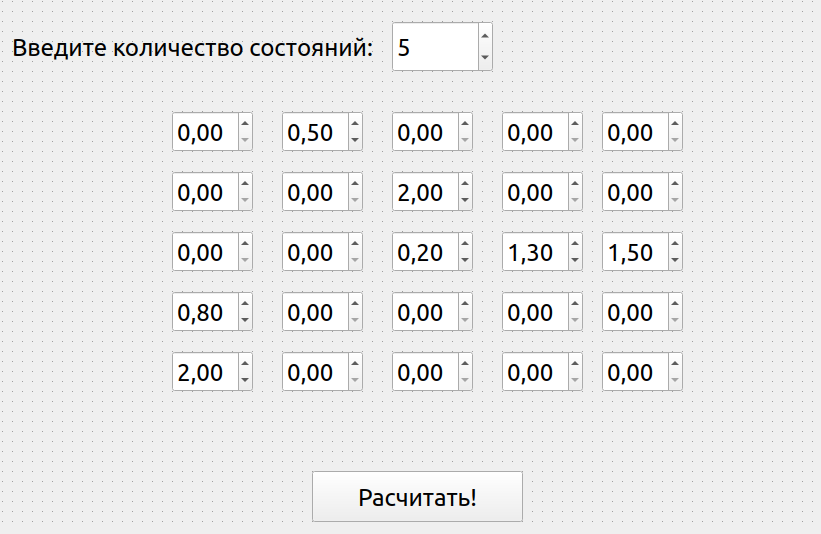
\includegraphics[width=\linewidth, height=10cm]{inc/demonstrate.png}
	\end{center}
	\caption{Демонстрация работы программы}
\end{figure}
\FloatBarrier

\newpage

Получившиеся результаты представлены в таблице 3:
\FloatBarrier
\begin{table}[h]
	\caption{Матрица интенсивности переходов в системе}
	\centering
	\begin{tabular}{| c | c | с | c | c | c |}
		\hline
		$p_{i}$  & 0.55172414 & 0.13793103 & 0.09195402 & 0.14942529 & 0.06896552 \\ \hline
		$t_{i}$  & 1.65 & 0.31 & 0.833 & 2.791 & 1.731 \\ \hline
	\end{tabular}
\end{table}
\FloatBarrier

График времени стабилизации вероятности состояний изображен на рисунке 2:
\FloatBarrier
\begin{figure}[h]
	\begin{center}
		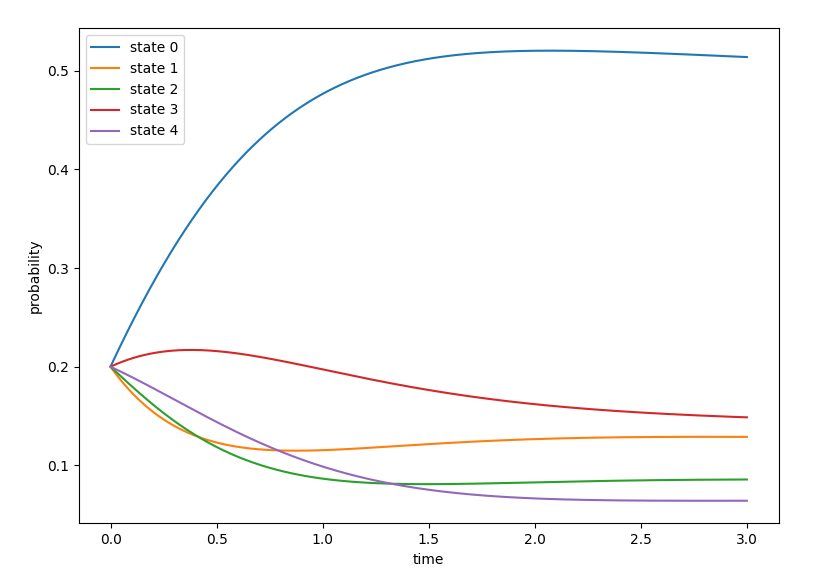
\includegraphics[width=\linewidth]{inc/graph.png}
	\end{center}
	\caption{Демонстрация работы программы}
\end{figure}
\FloatBarrier
